\documentclass[11pt,a4paper]{article}

\usepackage{microtype}
\usepackage{graphicx}
\usepackage{listings}
\usepackage{siunitx}
\usepackage{hyperref}
\usepackage{float}

\title{MPI Assignment}
\author{Jan van der Lugt}
\date{}

\begin{document}
\maketitle

\section{Introduction}
The report discusses my implementation of a parallel all-pairs shortest path (ASP) algorithm based on the famous Floyd-Warshall algorithm.

Section 2 explain will go through the implementation of the parallel version, while section 3 will report performance results, including a speedup graph and a table with execution times.

\section{Implementation}
The Floyd-Warshall ASP algorithm is very well and easily parallelizeable: every row has to be transmitted only once from its owner to all other processes, after which everyone uses this row to update distance values for their share of the distance table. This mimics the sequential execution, which can be seen as a special case of the parallel version with only one worker who is responsible for the entire table.

The calculation of the total road distance is also not very difficult to calculate: before the computation begins, every nodes sums up the entries in its part of the table (excluding MAX\_DISTANCE values), which are then combined using a sum reduction on the root. The same holds for the diameter of the road network, only this has to be calculated after the computation and using a maximum reduction.

To implement these features, various elements of MPI were used:
\begin{itemize}
\item To make it easier to send rows, a row type is defined as a contiguous block of $n$ integers. $n$ is first sent to all non-root processes using a MPI\_Bcast.
\item Rows are distributed among the processes using a MPI\_Scatterv, which takes an array of counts and displacements in order to distribute the table in one function call. The same is done at the end of the computation using MPI\_Gatherv. This required a slight change in the representation of the table in memory: in the sequential version, $n$ rows of size $n$ are allocated separately. In the parallel version, a block of $n$ x $n$ is allocated, after which pointers are created that point into this block.
\item MPI\_Reduce was used to reduce integers for the total road distance and road diameter.
\item MPI\_Bcast is used to send a row from its owner to all other processes at the start of every iteration of the computation.
\end{itemize}

\section{Performance results}
The cluster used for these experiments is the VU site of the DAS4, which consists of machines with dual Intel Xeon E5620 CPU's clocked at 2.40GHz. For the sequential version, one of these machines was used as well. For the parallel version, sets of 1, 2, 4, 8 and 16 machines were used. All runs were repeated 3 times.

Because the supplied test graphs were either too big to run in 15 minutes (chain\_10K.gr.new) or so small they ran in under a second (all the others), I chose to use randomly generated distance tables for the experiments. Only the computation time was measured, including the calculation of the total distance and the diameter. Data scattering and gathering time was excluded from this.

The way the distances are calculated is not dependent on the topology of the graph, as is the case for other algorithms, since the same amount of work is performed independent of the data in the table. Due to this, randomly generating a table using the built-in generator is representative for real-world graphs.

\begin{figure}[h]
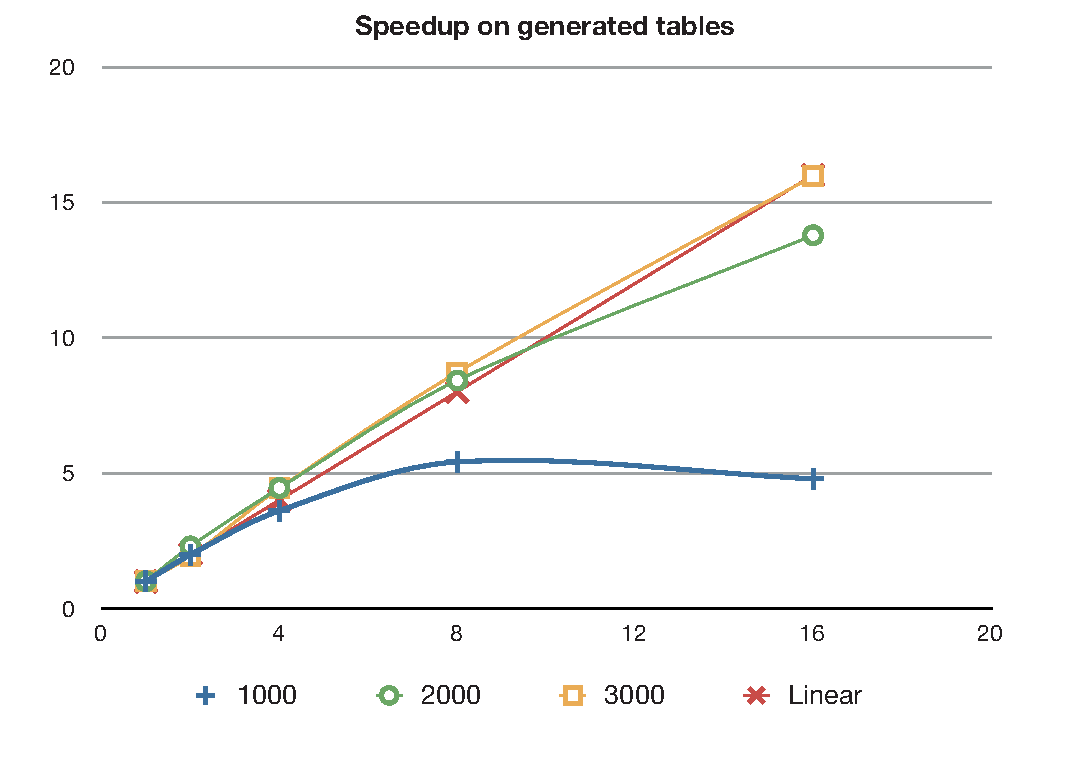
\includegraphics[scale=0.7]{figures/speedup.pdf}
\end{figure}

As we can see, the bigger the graph gets, the closer the speedup gets to linear speedup. For smaller graphs, there is too much overhead when they are processed by many (e.g. 16) workers.

Superlinear speedups can also be observed, this could be due to a larger part of the table fitting in caches. This is, however, merely a hypothesis.

\begin{tabular}{ | l | S | S | S | S | S | S | }
	\hline
	\textbf{Graph} & \textbf{Seq} & \textbf{Par 1} & \textbf{Par 2} & \textbf{Par 4} & \textbf{Par 8} & \textbf{Par 16} \\
	\hline                       
	test1.gr.new & 1,458 & 1,472 & 0,736 & 0,395 & 0,280 & 0,309 \\
	\hline
	test2.gr.new & 1,363 & 1,360 & 0,704 & 0,365 & 0,260 & 0,293 \\
	\hline
	test3.gr.new & 0,002 & 0,002 & 0,002 & 0,023 & 0,085 & 0,203 \\
	\hline
	test4.gr.new & 1,409 & 1,390 & 0,718 & 0,383 & 0,262 & 0,293 \\
	\hline
	Random (size 1000) & 1,452 & 1,451 & 0,731 & 0,402 & 0,268 & 0,303 \\
	\hline
	Random (size 2000) & 12,260 & 12,677 & 5,532 & 2,852 & 1,506 & 0,920 \\
	\hline
	Random (size 3000) & 39,959 & 40,841 & 21,234 & 9,206 & 4,689 & 2,559 \\
	\hline
\end{tabular} \\

It depends on the size of the table how large the cluster should be in order for the table to be processed in real-time. For a graph with 2000 vertices, a cluster of size 16 is fast enough. For a graph with 3000 vertices, a cluster of about 40 machines would probably be needed (2.5 times faster than 16 machines).

We can also observe that the parallel version almost always performs better than the sequential version, except for very small graphs like `test3.gr.new'.

\end{document}
